\chapter{Detection de régions d'intérêts }
\label{chap:regions}

Dans une collection d'images représentant un certains nombre d'objets, les prises de vue peuvent être multiples, de différents angles et à une distance pouvant variée. 
Il devient donc utile de s'intéresser à la position de l'objet dans l'image, que nous appelons région d'intérêt.
Faire un plongement uniquement sur la partie de l'image contenant l'objet permet d'éliminer les autres objets pouvant être présents sur l'image, par exemple des objets à peine visible ou hors mise au point.
Le plongement ainsi réalisé est plus à même de représenter correctement l'objet que le plongement de l'image entière.
Dans le cadre de notre projet, nous ne disposons pas d'annotation des régions d'intérêt dans les images (voir section~\ref{sec:contraintesGUIMUTEIC}). 
Ce chapitre propose une solution pour l'apprentissage de régions d'intérêts dans les images, de manière non supervisé et ne nécessitant pas d'annotation des régions au préalable et donc moins coûteux.

\section{Carte d'activation}

Des solutions à base de réseaux à proposition de régions (RPN pour Region Pooling Network) permettent une proposition automatique des régions par le réseaux. 
Les méthodes de l'état de l'art utilisant ce genre d'approche (section~\ref{sec:rpn}) obtienne une segmentation précise de l'image et une amélioration de la précision des plongements~\cite{gordo2016deep}.
Ces genre de méthodes nécessite toutefois un ensemble d'images annotées avec leurs régions pour fonctionner. 
Nous ne disposons pas d'une base de donnée annotées au niveau des régions. 
Ceci nous amène à développer des solutions ne nécessitant pas la présence de boîtes englobantes dans le corpus d'apprentissage.
Nous avons vu dans la section précédente qu'un apprentissage fin est nécessaire (étape 1 et 2 de la figure~\ref{fig:pipelinesimilarite}).
Ceci ne donne pas en soit des résultat suffisant pour l'identification d'instance, mais permet d'apprendre au réseau une certaine représentation des objets.

Le réseau est entraîné à reconnaître certain objets, et la sortie du réseau est dépendante de la présence ou non de ces objets dans les images.
Il a été montré~\cite{zhou2014object} que lorsqu’un réseau est appris sur une collection, il est capable d’identifier la présence de certains objets, même s’il ne les classifie pas explicitement.
Ce qui signifie que si l’on applique notre réseau sur chaque sous partie de l’image, on obtient des maximum d’activation du réseau, si un des objets qu’il a appris à reconnaître est présent.
On prenant les zones où les réseau a des activations plus importante, on peut créer une carte des activations du réseau.
Ces cartes d’activations sont présentés sur la figure~\ref{fig:heatmaps}.
Un réseau de type ResNet, après un apprentissage fin sur la collection, est appliqué sur un certain nombre de sous partie de l’image.
Les zones en rouge sur les cartes d’activations représentent les endroits où les maximum d’activation était les plus important.
On remarque que ces zones correspondent aux emplacements des objets, avec quelques erreurs sur le troisième tableau.
On voit dans la troisième colonne la classification de chacune de ces sous-partie.
Cette classification n’est pas correcte, avec des labels erronés, et très variés. 
Ces résultats sont en relation avec les résultats relativement faibles obtenu dans le chapitre précédent avec la classification, 79\% contre 92\% pour l’extraction de caractéristiques. 
En revanche, cette méthode permet d'identifier les régions d'intérêt de l'image.

\begin{figure}[!htb]
  \centering
  \begin{minipage}[c]{.33\linewidth}
    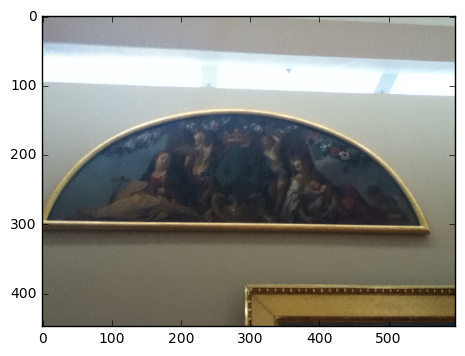
\includegraphics[width=\textwidth]{figures/sample1_10A-0519.png}
    %\caption{Image with label 10A\label{fig:sample1_id}}
  \end{minipage} \hfill
  \begin{minipage}[c]{.33\linewidth}
    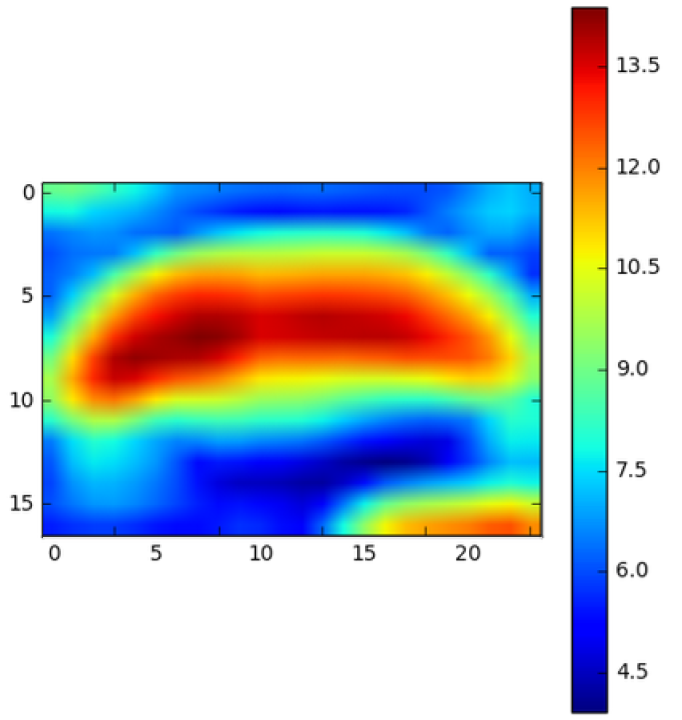
\includegraphics[width=\textwidth]{figures/sample1heatmap.png}
    %\caption{Heat-map for 10A\label{fig:sample1_hm}}
  \end{minipage} \hfill
  \begin{minipage}[c]{.32\linewidth}
    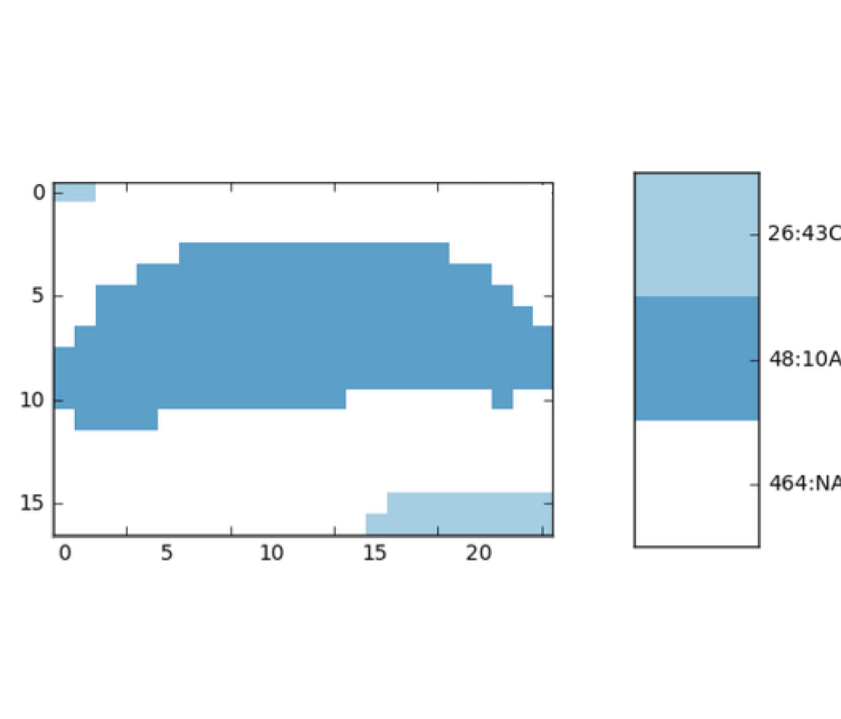
\includegraphics[width=\textwidth]{figures/sample1labels.png}
    %\caption{Label-map for 10A\label{fig:sample1_lab}}
  \end{minipage}

  \begin{minipage}[c]{.33\linewidth}
    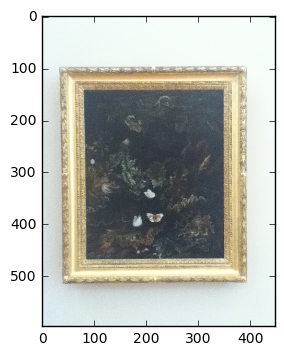
\includegraphics[width=\linewidth]{figures/sample2_5P-0508.png}
    %\caption{Image with label 5P\label{fig:sample2_id}}
  \end{minipage} \hfill
  \begin{minipage}[c]{.33\linewidth}
    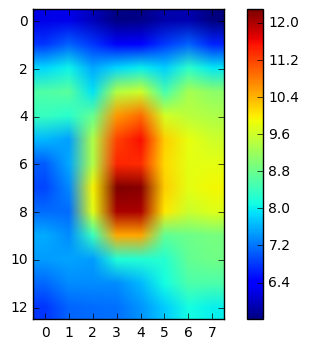
\includegraphics[width=\linewidth]{figures/sample2_heatmap.png}
    %\caption{Heat-map for 5P\label{fig:sample2_hm}}
  \end{minipage} \hfill
  \begin{minipage}[c]{.32\linewidth}
    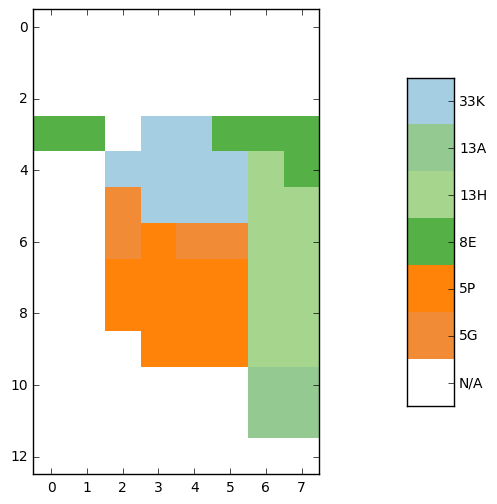
\includegraphics[width=\linewidth]{figures/sample2_labels.png}
    %\caption{Label-map for 5P\label{fig:sample2_lab}}
  \end{minipage}
  
  \begin{minipage}[c]{.33\linewidth}
    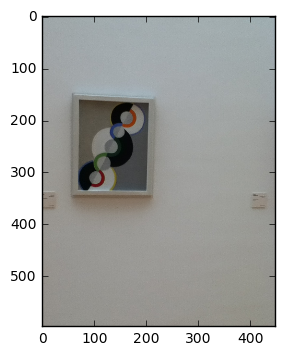
\includegraphics[width=\linewidth]{figures/sample3_30P-0976.png}
    %\caption{Image with label 30P\label{fig:sample3_id}}
  \end{minipage} \hfill
  \begin{minipage}[c]{.33\linewidth}
    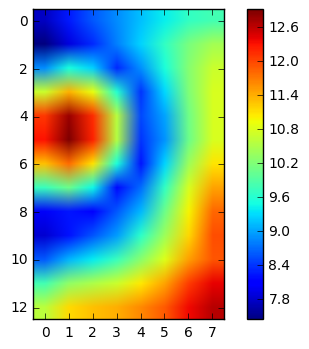
\includegraphics[width=\linewidth]{figures/sample3_heatmap.png}
    %\caption{Heat-map for 30P\label{fig:sample3_hm}}
  \end{minipage} \hfill
  \begin{minipage}[c]{.32\linewidth}
    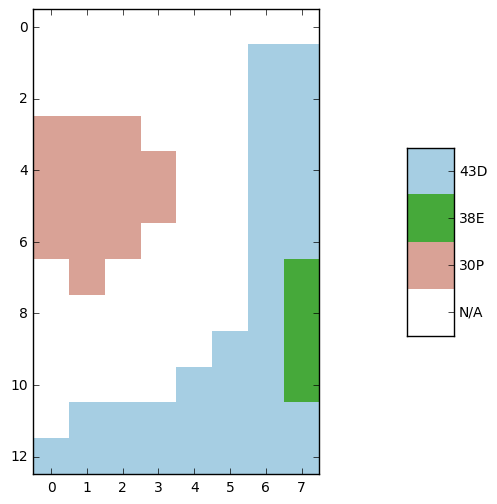
\includegraphics[width=\linewidth]{figures/sample3_labels.png}
    %\caption{Label-map for 30P\label{fig:sample3_lab}}
  \end{minipage}


	\caption{Exemple d'images avec les heat-map des activations maximales, obtenues à partir d'un ResNet-152 après un apprentissage fin. Le réseau est appliqué sur toute l'image de manière strié. Les labels obtenus sur les zones d'activation maximales sont également indiqués.
	\label{fig:heatmaps}}
	
\end{figure}



Le problème avec l'application d'un réseau d’une telle manière est le coût de calcul.
Par exemple, temps de passage d'une image $224*224$ à travers AlexNet est de 1.2 ms. 
Si on applique ce même réseau sur une image $448*448$ avec un pas de 56 pour créer une carte d’activation de $8*8$, il faut 76.8 ms.

Cette méthode n’est donc pas envisageable, surtout s’il on souhaite utiliser des images plus grande pour obtenir une carte d'activation plus précise.
La solution est d’utiliser des réseaux entièrement convolutifs.
Dans la section~\ref{sec:rpn}, nous avons vu que les réseaux entièrement convolutifs pouvaient être utilisés pour la segmentation d'image.
Dans le cas où nous n'avons pas de base données d'apprentissage de la segmentation, nous entraînons le réseau comme expliqué précédemment, et nous remplaçons les couches entièrement connectées par une couche de convolution.
Il y a une équivalence entre une couche entièrement connectée et une couche de convolution $1*1$, comme montré sur le schéma~\ref{fig:equivalencecouche}, avec le même nombre de paramètres.
L'avantage de la couche de convolution est que l'on peut l'appliquer sur n'importe quelle taille d'image (figure~\ref{fig:convBig}), la taille de sortie dépendant de la taille d’entrée.
Le temps d'exécution d’un réseau type AlexNet entièrement convolutionnel sur une image de $448*448$ est de 18 ms, soit 5 fois plus rapide que l’approche naïve.



\begin{figure}[htbp]
\begin{subfigure}{0.32\textwidth}
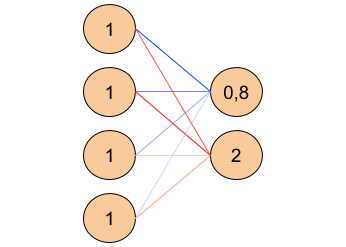
\includegraphics[width=\linewidth]{figures/LinearLayer(1).png}
\caption{Couche Entièrement connectée} \label{fig:linear}
\end{subfigure}
\hspace*{\fill} % separation between the subfigures
\begin{subfigure}{0.32\textwidth}
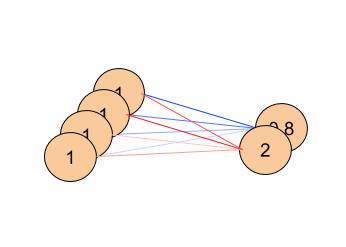
\includegraphics[width=\linewidth]{figures/FConvolutional(1).png}
\caption{Couche de convolution} \label{fig:conv}
\end{subfigure}
\hspace*{\fill} % separation between the subfigures
\begin{subfigure}{0.32\textwidth}
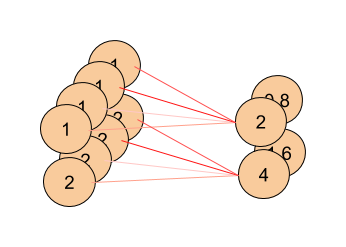
\includegraphics[width=\columnwidth]{figures/FConvolutional2(1).png}
\caption{Même couche de convolution avec entrée plus grande} \label{fig:convBig}
\end{subfigure}
\caption{Exemple d'équivalence entre une couche entièrement connectée et une couche de convolution. Le nombre de paramètres est le même, ici $4*2$, ils peuvent donc être copié pour obtenir les mêmes résultats. On peut appliquer la convolution avec une entrée plus grande, en une seule passe.} 
\label{fig:equivalencecouche}
\end{figure}



\section{Apprentissage sur différentes régions}

L'approche présentée précédemment permet de mettre en avant qu'il est possible de détecter les régions sans apprentissage direct de celles-ci.
Nous pouvons toutefois améliorer les résultats de la détection de régions d'intérêt en faisant un apprentissage fin sur des régions spécifique de l'image, plutôt que sur l'image entière.
En utilisant différentes échelles et différentes régions, toujours pour apprendre la même classe, nous pouvons forcer le réseau à détecter les régions dans l'image.
La fonction de coût associé à cette apprentissage est la moyenne de l'entropie croisée entre les régions et entre les échelles. 
Dans le cas de la classification, l’étiquette d'une image, qui représente sa classe, est un vecteur $\hat{x}$ de dimension $C$, où $C$ est le nombre de classes, où chaque éléments $\hat{x}_i$ est à zéro si la classe $i$ n'est pas présente, $1$ sinon.
La sortie du réseau de neurones $x$ est une distribution de probabilité pour chaque classe.
L'entropie croisée $E$ est définie par :

\begin{equation}
  E(x,\hat{x}) = -\sum_{i=1}^C \hat{x}_i log(x_i)
	\label{eq:entropie2}
\end{equation}

Pour une image à une échelle $s$ donnée, définissons $H_s$ et $W_s$ comme respectivement la hauteur et la largeur de la carte de caractéristiques.
Chaque pixel de la carte d'activation correspond à un sortie du réseau de neurones pour une région de l'image donnée.
Le nombre de région est donc $H_s*W_s$. 
Nous notons $x_{h,w}$ la distribution de probabilité (la sortie du réseau) sur la région $(h,w)$.
Nous définissons la fonction objectif suivante:

\begin{equation}
 \mathcal{L}(x,\hat{x}) = \frac{1}{S} \sum_{s=1}^S \frac{1}{H_s*W_s} \sum_{h=1}^{H_s} \sum_{w=1}^{W_s} E(x_{h,w}, \hat{x}_{h,w})
\label{eq:regionloss}
\end{equation}

qui représente la moyenne de l'entropie croisée de l'ensemble des régions, moyennée sur l'ensemble des échelles de l'image.
La figure~\ref{fig:regionfinetuning} représente l'apprentissage avec cette fonction objectif. 
L'idée étant de forcer le réseau de neurones à se concentrer sur certaines régions, pour classifier l'image.


\begin{figure}[!htb]
\centering
    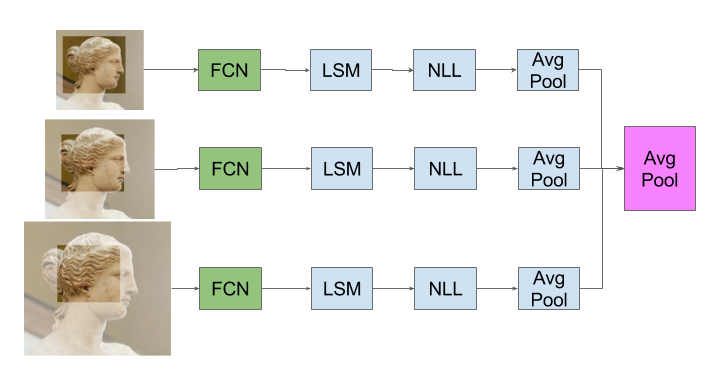
\includegraphics[width=\linewidth]{figures/Average_Loss.png}
    \caption{Calcul de la fonction de coût lorsque l'on entraîne le réseau sur différentes régions à différentes échelles. L'entropie croisée $E$ est calculé pour chaque segment d'image avant d'être moyenné (equation.~\ref{eq:regionloss}).
    \label{fig:regionfinetuning}}
\end{figure}


\section{Apprentissage de régions et de similarité}

Une fois l'apprentissage sur les régions réalisé, nous disposons d'un réseau capable de se focaliser sur une certaine région de l'image.
Nous utilisons ceci pour changer la fonction objectif triple.
Celle définie précédemment (équation~\ref{eq:objectif}) ne prend pas en compte les régions.
Si l'on prend en compte comme région d'intérêt les $k$ éléments avec la plus forte activation du réseau, on peut extraire les caractéristiques depuis uniquement cette zone, qui représente la région la plus probable de présence de l'objet.
Pour la fonction objectif de l'apprentissage, en plus du plongement correct des images positives et négatives, nous ajoutons la classification de cette région avec l'entropie croisée.
Ce qui donne l'équation suivante :

\begin{equation}
\mathcal{L}(x,y,z,\hat{x}) =  \alpha \max(0, x \cdot z - x \cdot y + m) +
(1-\alpha) \frac{1}{k} \sum_{l=1}^k E(x_{h,w}, \hat{x}_{h,w})
\label{eq:proposedloss}
\end{equation}

On retrouve le plongement des images $x,y$ et $z$, qui doivent vérifier l'objectif triple (équation~\ref{eq:objectif}.
Ainsi que la classification des $k$ région de plus forte activation, avec $\alpha$ la régularisation entre les deux objectifs de la fonction de coût.

Dans le but de réaliser cette onction, nous définissons un réseau de neurones entièrement convolutif, capable de produire une sortie de classification de la région de plus grande activation, ainsi qu'un plongement de cette région.
Pour ce faire, une couche de ``pooling'' des $k$ régions de plus forte activation est ajouté à la sortie du réseau. 
En s'inspirant de l'architecture R-MAC~\cite{gordo2016deep}, une normalization $L2$, un décalage et une couche entièrement connectée sont ajoutés à cette sortie.
Ce pipeline permet de réaliser une PCA (Principal Component Analysis) pour réduire la taille de la représentation~\cite{jegou2012negative}.
Les paramètres du décalage sont appris par rétro-propagation et la couche entièrement connecté permet de réduire la taille du descripteur à la taille désirée pour l'espace de projection $\mathbb{E}$.
Une normalisation $L2$ est de nouveau opérée pour normaliser le plongement des images.

\begin{figure}[!htb]
\centering
    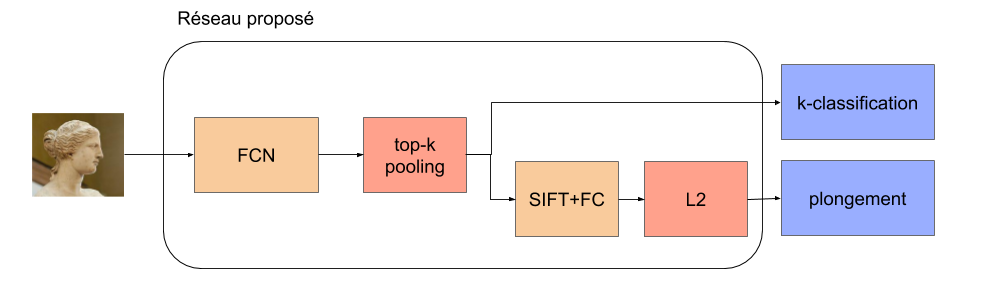
\includegraphics[width=\linewidth]{figures/ProposedNetwork.png}
    \caption{Architecture du réseau proposé basé sur un réseau entièrement connecté pré-entrainé pour détecter les régions d'intérêt.
    \label{fig:proposednetwork}}
\end{figure}

Pour l'entraînement de ce réseau, nous utilisons une architecture à trois branches comme précédemment, à laquelle nous ajoutons la classification des $k$ régions de plus fortes activation, comme montré sur le schéma~\ref{fig:finalpipeline}.
La même stratégie de sélection des triplets que celle utilisée précédemment est appliquée.

%\begin{figure}[!htb]
    %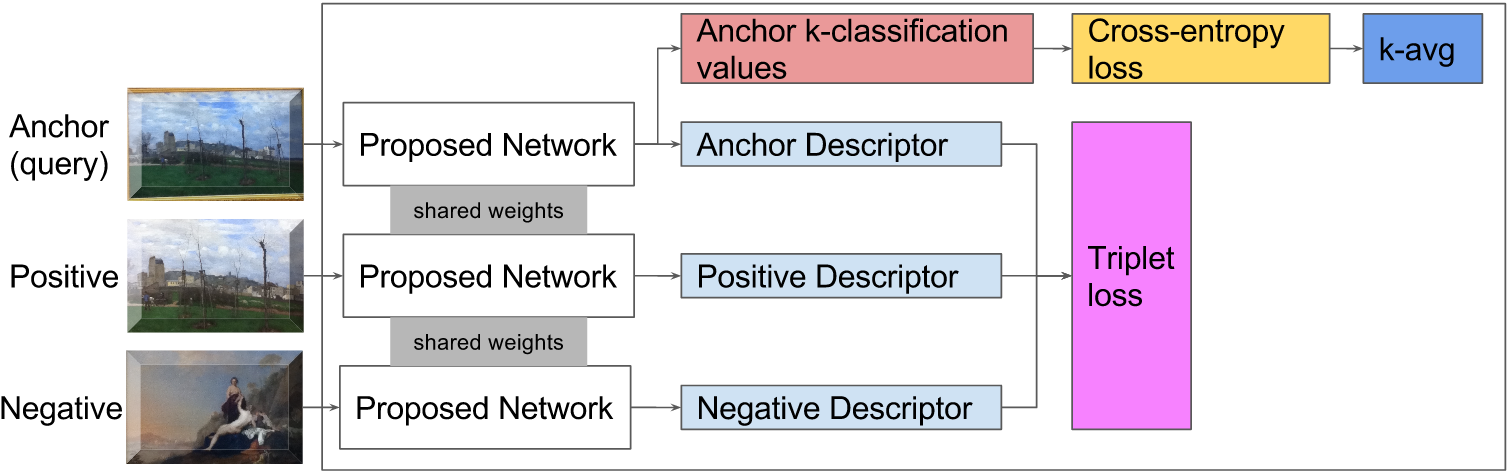
\includegraphics[width=\linewidth]{figures/contrib_train.png}
    %\caption{CORRECT MAIS A REFAIRE CAR NOTATION INCORRECT Proposed architecture for instance search based on an FCN ~\cite{long_fully_2015} for region proposals, at training time
    %\label{fig:contribtrain}}
%\end{figure}

La figure~\ref{fig:finalpipeline} reprend l'ensemble des étapes de l'apprentissage, en incorporant l'apprentissage des régions. 
Les étapes 1 et 2 sont identiques à celles présenté au chapitre précédent.
L'étape 3 correspond à l'apprentissage des régions d'intérêt.
Enfin, l'étape 4 est l'apprentissage grâce à la fonction de coût~\ref{eq:proposedloss}.	
\begin{figure}%
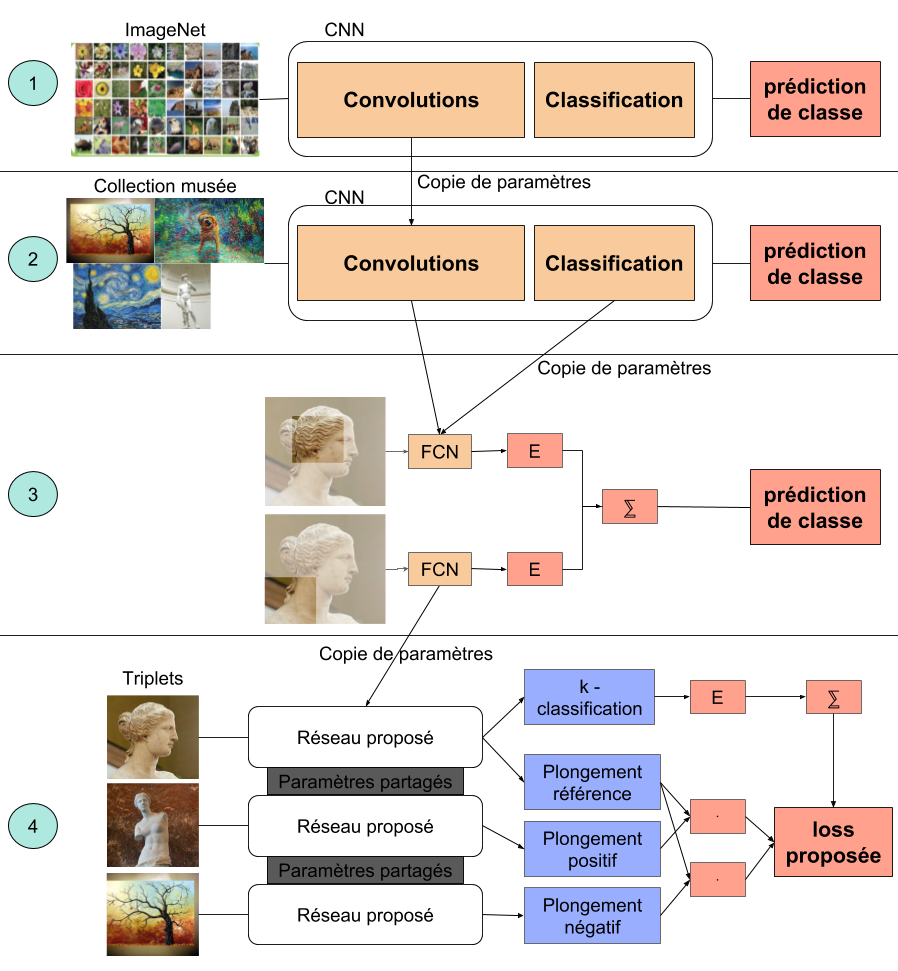
\includegraphics[width=\columnwidth]{figures/pipelinefinal.png}%
\caption{Pipeline final d'apprentissage, avec l'ajout de la détection des régions d'intérêts.}%
\label{fig:finalpipeline}%
\end{figure}


\section{Expérimentation}

Nous testons notre approche sur deux collections du projet GUIMUTEIC, CLICIDE et GaRoFou, et nous évaluons grâce au métriques suivantes :
\begin{itemize}
	\item La précision à 1 (TOP@1) : l'image la plus proche contient le même objet.
	\item La précision moyenne (MAP pour Mean Average Precision) : la moyenne des valeurs de précision des images pertinentes (contenant le même objet) dans la liste ordonnée en fonction des distances.
\end{itemize}






\subsection{Paramètres d'apprentissage}

Pour les premières étapes de l'apprentissage, les mêmes paramètres que dans le chapitre précédent sont utilisés, commes les étapes 1 et 2 sont identiques.
La sélection des triplets se fait également de la même manière que précédemment, à savoir : dans un premier temps tous les triplets négatifs semi-difficiles, puis tous les triplets négatifs difficiles.

Comme nous utilisons un réseau entièrement convolutif, la taille des images pour l'apprentissage est libre, contrairement à un réseau contenant des couches entièrement connectées.
Pour nos expérimentation, nous utilisons une taille fixe pour la plus petit côté des images en entrée, avec deux échelles différentes.
Pour ResNet, nous utilisons deux échelles : $448$ et $224$.
Pour AlexNet, nous avons trouvé que la convergence n'était pas correcte avec les mêmes paramètres, nous utilisons donc les échelles : $384$ et $224$.
Lorsque l'on utilise des images avec des ratio entre hauteur et largeur très grand, l'utilisation de mémoire pendant l'apprentissage peut être très importante. 
Pour limiter cela, nous limitons le ratio au maximum à $2.0$.

Les paramètres de la fonction de coût~\ref{eq:proposedloss} sont $\alpha = 0,5$ et $k=6$.

%The stride of a full network depends on the architecture and is 32
%pixels for the architectures used here: AlexNet and ResNet.
%
%For the processing of the Fully Convolutional networks (step 2 of our proposal, described in part~\ref{sec:contrib}), all images are scaled to have the same number of pixels in the smaller side in order to normalize the sizes of the features present in the images. 
%Note that for large aspect ratios and large scales of the smaller side, the memory consumption of training can be high for single images having a very large aspect ratio.  To limit this spike in memory consumption, the aspect ratios are limited by introducing uniform random noise on the smaller side of images with high aspect ratios. In our experiments, we use a maximal aspect ratio of $2.0$ and images
%at two scales of $448$ and $224$ pixels for the smaller side. We found
%that the AlexNet architecture did not have good convergence behavior,
%thus we used scales of $384$ and $224$ instead.



\subsection{Résultats}
\label{sec:resultatregion}

\begin{table*}
\centering
\begin{tabular}{|l||c|c||c|c|}
\hline & \multicolumn{2}{c||}{\emph{top@1 (en \%)}} &
\multicolumn{2}{c|}{\emph{MAP (en \%)}}\\
\hline & \emph{CLICIDE} & \emph{GaRoFou} & \emph{CLICIDE} & \emph{GaRoFou}\\
\hline \emph{Gordo multi-res~\cite{gordo2016deep}}
& 92.73 & 95.65 & 65.49 & 89.32\\ \hhline{|=||=|=||=|=|}
\hline \emph{AlexNet E} & 72.73 & 85.87 & 32.71 & 66.11\\
\hline \emph{AlexNet Classif} & 78.18 & 90.76 & 38.51 & 72.92\\
\hline \emph{AlexNet SS} & 75.76 & 90.20 & 36.20 & 77.73\\
\hline \emph{AlexNet + Régions} & 81.21 & 83.15 & 45.53 & 71.71\\ 
\hhline{|=||=|=||=|=|}
\hline \emph{ResNet E} & 72.12 & 85.33 & 40.99 & 70.15\\
\hline \emph{ResNet Classif} & 79.39 & 94.57 & 75.11 & \textbf{93.44}\\
\hline \emph{ResNet SS} & 85.45 & 95.11 & \textbf{83.00} & 91.90\\
\hline \emph{ResNet + Régions} & \textbf{94.55} & \textbf{96.20}
& 82.94 & 91.83\\
\hline
\end{tabular}
\caption{TOP@1 et MAP des différentes approches sur les collections CLICIDE et GaRoFou.
\label{tab:results}}
\end{table*}



Le tableau~\ref{tab:results} présente les résultats obtenu sur CLICIDE et GaRoFou par l'approche proposée, comparé aux approches précédentes.
Nous remarquons que notre méthode obtient le meilleur TOP@1, avec un score de 94.55\% comparé aux 92.73\% de l’état de l’art sur CLICIDE.
Sur GaRoFou, les méthodes de l’état de l’art obtiennent un score de 95.65\%, le gain est moins important, avec 0.55\%.
Comme montré précédemment, ResNet présente toujours de meilleurs résultats que AlexNet.
L'apport de la propositions de régions par le réseau, même sans base d'apprentissage annotées, permet donc d'améliorer les résultats.
Toutefois, si l'on s'intéresse à la MAP, on voit qu'aucune des méthodes proposées ne permet d'obtenir de meilleurs résultats qu'un réseau Siamois Simple (SS), où qu'un fine-tuning dans le cas de GaRoFou (Classif).
Cela nous amène à penser que même si le TOP@1 est bon, l'espace de projection créé ne capture pas complètement la similarité entre les images.



\section{Indexation et augmentation de données côté base de données}

Pour l'identification d’instance, nous utilisons la recherche du plus proche voisin dans la base de données d’image.
Un parcours simple de cette base de donnée est suffisant, étant donné la taille de nos collection.
On peut même augmenter le nombre d’éléments dans la base de données, ce qui est nommé ``Database-side feature augmentation''~\cite{turcot_better_2009,arandjelovic_three_2012}.
Cela permet d’améliorer la recherche, en couvrant plus l’espace de recherche.

Pour modifier les éléments dans l’espace de projection, il y a deux stratégies : soit ajouter des points dans l'espace, soit de changer le plongement de chaque élément de la base de données.
On peut par exemple remplacer chaque éléments de l'espace par une combinaison de ces $k$ plus proches voisins, ce qui permet de lisser les projections, et de corriger le bruit~\cite{gordo2016deep}. 
Dans notre cas, nous disposons généralement de peu d'image références pour chaque objet, nous n'envisageons donc pas de modifier les plongement en fonction de leur voisin, mais plutôt de créer de nouvelles projections, pour rendre l'espace plus dense.

Pour l’ensemble des exemples d’une instance, nous prenons chacun des plongements, et calculons leur moyenne.
Ce nouveau vecteur peut être considéré comme un nouvel exemple pour l'instance donnée.
Nous pouvons donc l'ajouter à l'espace de projection.
Ce nouveau point peut également servir de référence pour l’instance qu’il représente, ce qui permet de supprimer tous les autres éléments de l’espace.
Ainsi, le nombre d'éléments à parcourir pour la recherche du plus proche voisin n’est plus l’ensemble des exemple, mais uniquement un pour chaque instance.


 %proposes to combine descriptors of the reference images in order to form better database-side descriptors.
%Every reference descriptor is simply replaced by a combination of itself and the $k$ nearest neighbors. 
%This combination is computed as a weighted sum, weighted by the rank of the neighbors with respect to $k$ (the closest neighbor has the highest weight and the $k$-th neighbor the lowest).
%
%In our work, we use a technique called Instance Feature Augmentation.
%We use the fact that we know the corresponding label for each image in our dataset.
%For each label, we compute the representation of an instance by averaging the features of every images corresponding to this label. 
%This representation is added to the dataset as a new instance.
%We show that this approach does not improve mean precision@1, but gives a better Mean Average Precision. 
%This suggests that the internal representation of the instance is improved. 

Le tableau~\ref{tab:resultsAugmentation} montre les résultats obtenu avec l'augmentation de données de la base de donnée par rapport au résultats précédents.
L'ajout de l'augmentation de donnée n'améliore pas le top@1, voir même la détériore, avec en moyenne une perte de 0.5\%.
Par contre, on remarque une nette amélioration de la MAP, ce qui signifie que les nouveaux exemples créé dans la base de donnée capture bien certaines instances.

\begin{table*}
\centering
\begin{tabular}{|l||c|c||c|c|}
\hline & \multicolumn{2}{c||}{\emph{TOP@1 (en \%)}} &
\multicolumn{2}{c|}{\emph{MAP (en \%)}}\\
\hline & \emph{CLICIDE} & \emph{GaRoFou} & \emph{CLICIDE} & \emph{GaRoFou}\\
\hline \emph{AlexNet proposé} & 81.21 & 83.15 & 45.53 & 71.71\\
\hline \emph{AlexNet proposé + Augmentation} & 80.61 & 82.61 & 71.02 & 81.66\\ 
\hhline{|=||=|=||=|=|}
\hline \emph{ResNet proposé} & \textbf{94.55} & \textbf{96.20}
& 82.94 & 91.83\\
\hline \emph{ResNet proposé + Augmentation} & 93.94 & 95.11
& \textbf{94.23} & \textbf{93.86}\\
\hline
\end{tabular}
\caption{TOP@1 et MAP sur les corpus CLICIDE et GaRoFou, avec et sans l'augmentation de données coté base de données.}
\label{tab:resultsAugmentation}
\end{table*}


\begin{figure}
  \centering
  \begin{minipage}[c]{.33\linewidth}
    \centering
    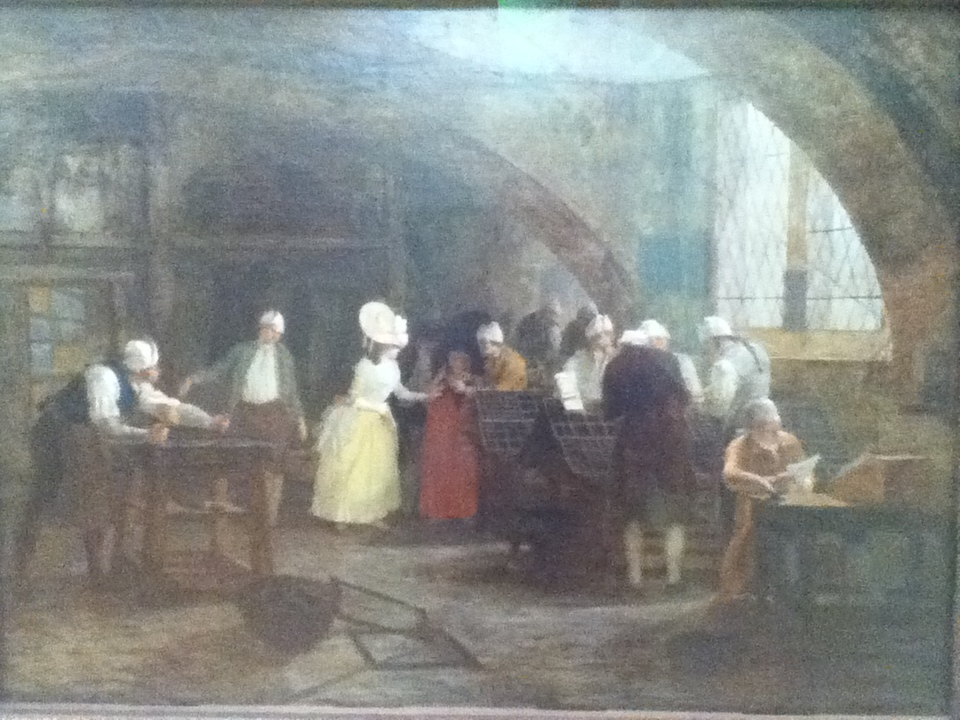
\includegraphics[width=\textwidth]{figures/11J-0521.JPG}
  \end{minipage} \hfill
  \begin{minipage}[c]{.33\linewidth}
    \centering
    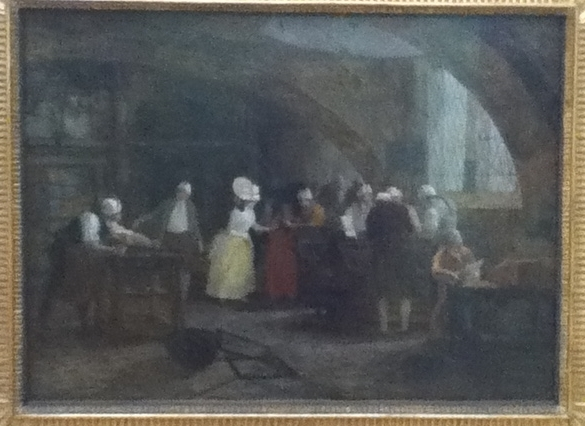
\includegraphics[width=\textwidth]{figures/11J-1.JPG}
  \end{minipage}
  \begin{minipage}[c]{.32\linewidth}
    \centering
    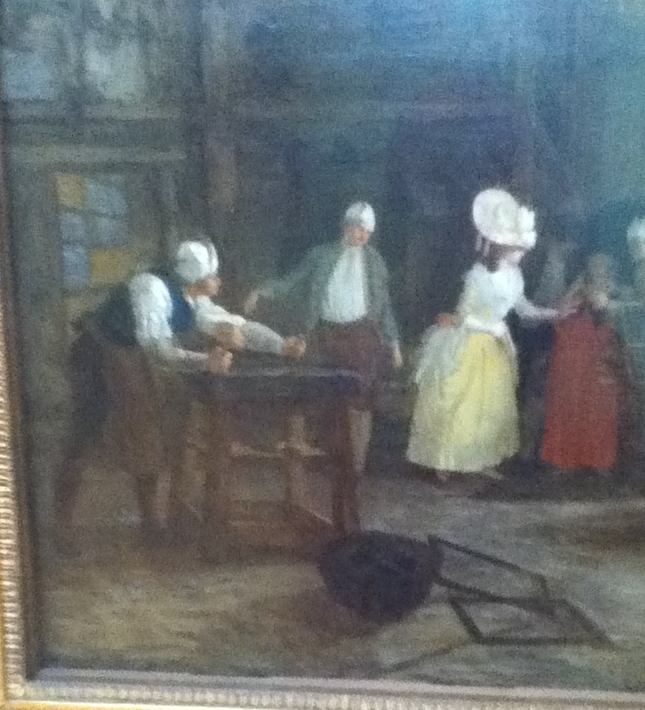
\includegraphics[width=\textwidth]{figures/11J-4.JPG}
    %\caption{Heat-map for 10A\label{fig:sample1_hm}}
  \end{minipage}

  \begin{minipage}[c]{.33\linewidth}
    \centering
    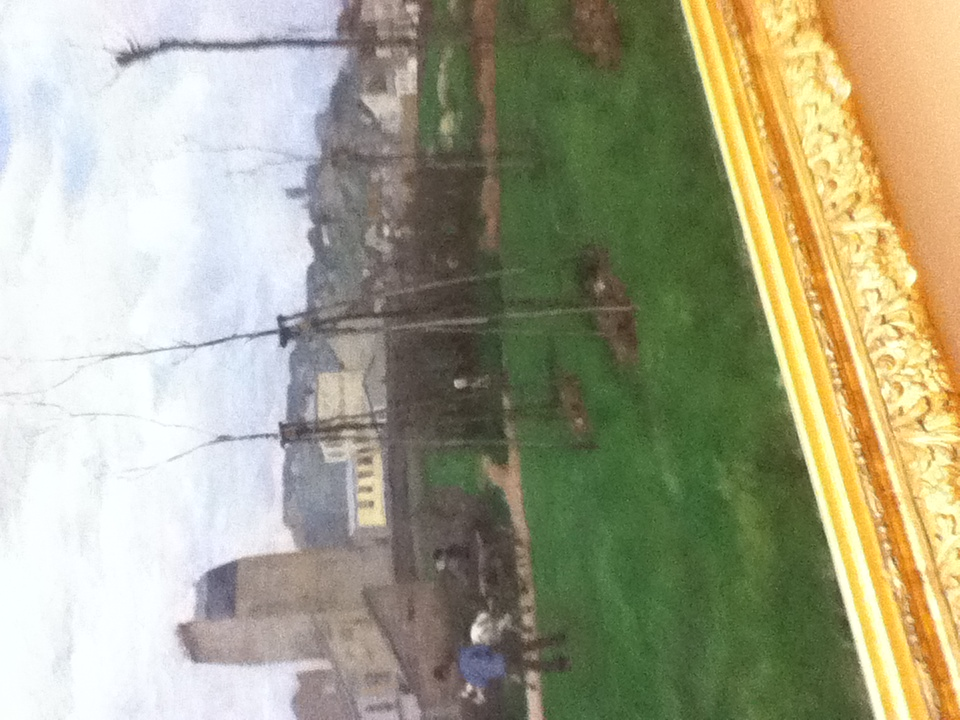
\includegraphics[width=\textwidth, angle=270]{figures/23D-0740.JPG}
  \end{minipage} \hfill
  \begin{minipage}[c]{.33\linewidth}
    \centering
    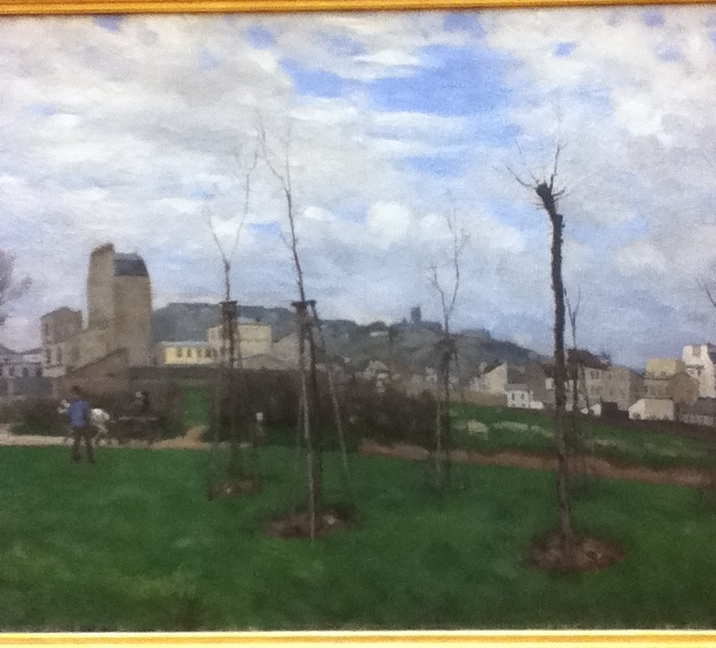
\includegraphics[width=\textwidth]{figures/23D-2.JPG}
  \end{minipage}
  \begin{minipage}[c]{.32\linewidth}
  	\centering
    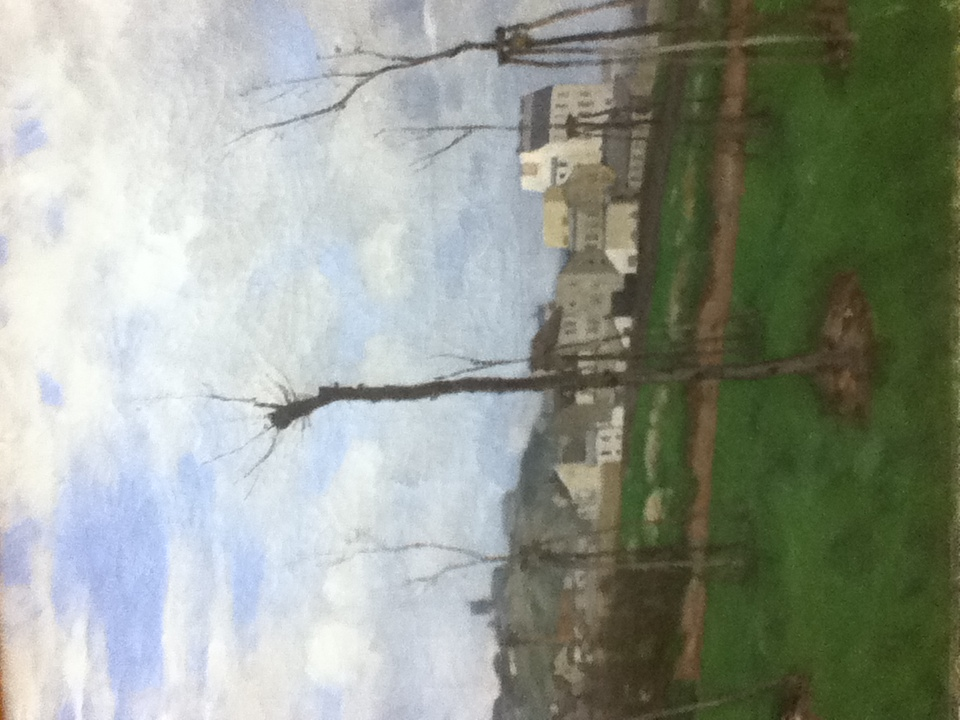
\includegraphics[width=\textwidth, angle=270]{figures/23D-1.JPG}
    %\caption{Heat-map for 10A\label{fig:sample1_hm}}
  \end{minipage}
  
  \begin{minipage}[c]{.33\linewidth}
    \centering
    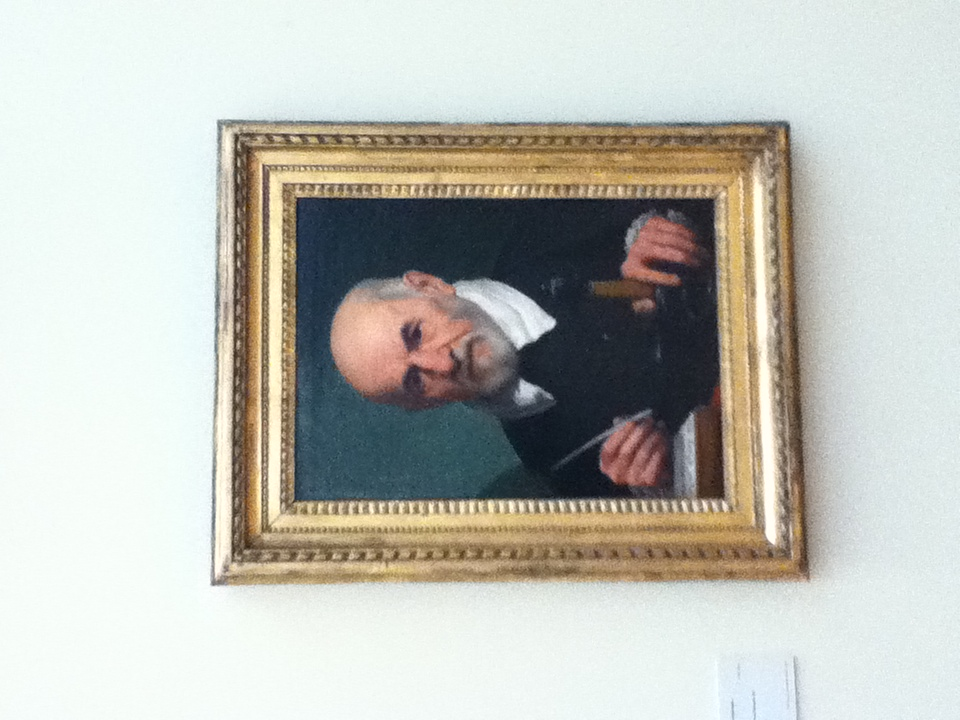
\includegraphics[width=\textwidth, angle=270]{figures/1C-0454.JPG}
  \end{minipage} \hfill
  \begin{minipage}[c]{.33\linewidth}
    \centering
    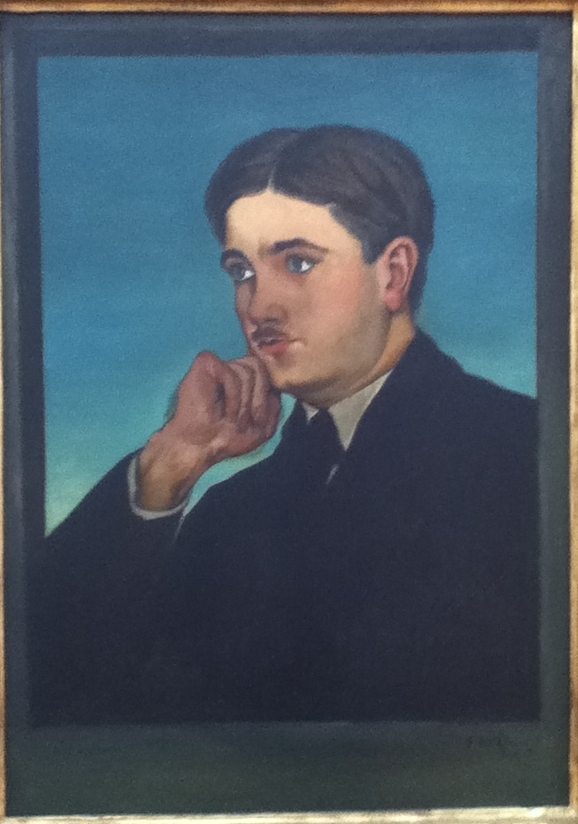
\includegraphics[width=\textwidth]{figures/1.png}
  \end{minipage}
  \begin{minipage}[c]{.32\linewidth}
    \centering
    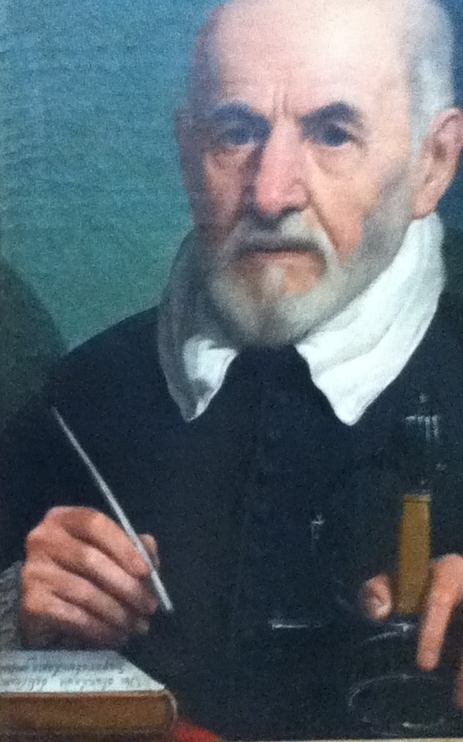
\includegraphics[width=\textwidth]{figures/1C-0.JPG}
    %\caption{Heat-map for 10A\label{fig:sample1_hm}}
  \end{minipage}
  
  
  \begin{minipage}[c]{.33\linewidth}
    \centering
    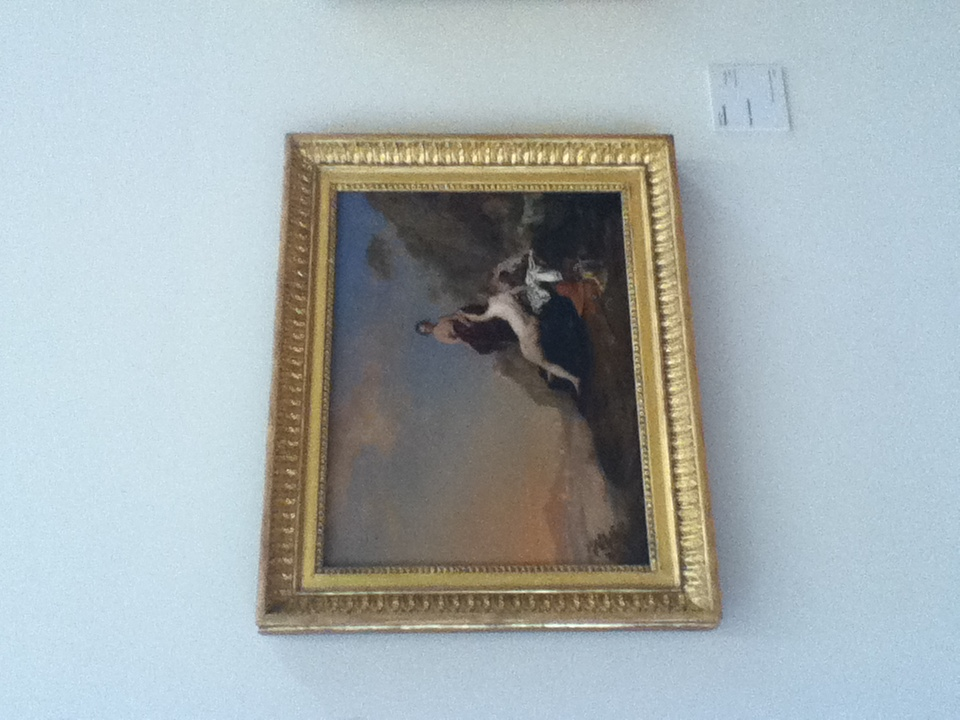
\includegraphics[width=\textwidth, angle=270]{figures/5B-0506.JPG}
  \end{minipage} \hfill
  \begin{minipage}[c]{.33\linewidth}
    \centering
    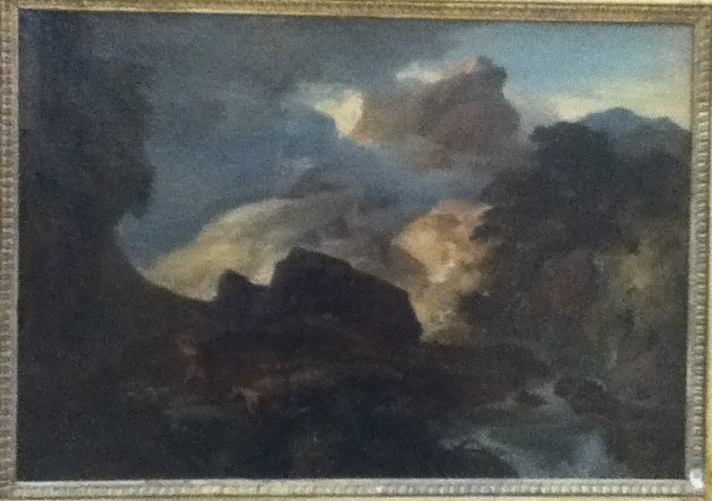
\includegraphics[width=\textwidth]{figures/2.png}
  \end{minipage}
  \begin{minipage}[c]{.32\linewidth}
    \centering
    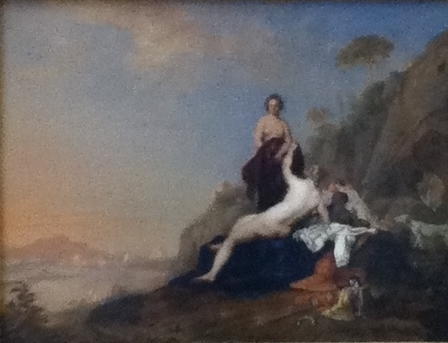
\includegraphics[width=\textwidth]{figures/5B-0.JPG}
    %\caption{Heat-map for 10A\label{fig:sample1_hm}}
  \end{minipage}
  
\caption{Exemples de succès et d'échecs de notre approche. La première colonne représente les requêtes, les deuxième colonne contient les images les plus proches et la troisième colonne la deuxième image la plus proche dans la collection CLICIDE.}
\label{fig:failing}
\end{figure}

La figure~\ref{fig:failing} montre quelques exemples de succès et d'échecs de notre approche.
Pour chaque requêtes (colonne de gauche), on affiche les deux images les plus proches.
On remarque que dans les échecs, la deuxième image retournée est la bonne (la TOP@2 est de 100\%).
L'augmentation de données dans l'espace de projection permet donc de créer un espace plus dense, qui capture mieux la similarité entre les images.
Même si cela n'améliore pas la TOP@1 dans notre cas, cela permet d'envisager d'autre approches pour la détection d'instance, notamment si l'on s'intéresse aux vidéos, avec par exemple un vote majoritaire ou une moyenne des instances retournées.

Notre approche permet donc d'obtenir de meilleurs résultats que les méthodes de l'état de l'art, dans le cas des corpus de petites tailles.
Notre solution d'apprentissage de régions non supervisé permet d'avoir une proposition de régions d'intérêts par le réseau.
La proposition de régions pour la création du plongement semble être un point clef pour la recherche d'instance dans les images.
Enfin, une densification de l'espace de projection par augmentation de données permet de mieux capturer la similarité entre les images dans l'espace de projection, avec cependant une perte en précision.




